% !TeX root = ../main.tex

\chapter{项目总结}
\label{cha:chapter04}
本文设计并实现了一种进行跳跃滑翔运动的机械装置。该机器人能够完成设定的伸腿及展翅动作,但由于无感启动的原理性不足与腿部连接的材料缺陷,未能按设计实现跳跃滑翔功能。根据实验结果,在第\ref{cha:chapter03}章的结尾给出了该项目可行的改进方向,可使机器人达到更好的性能,实现跳跃滑翔的原定运动目标。总结如下:
\begin{itemize}
  \item 增加霍尔传感器,对电机进行力矩控制;
  \item 对腿部连接件进行重新设计,减小晃动;
  \item 增加额外的自由度对身体重心进行控制。
\end{itemize}

~\\
\begin{figure}[h]
  \centering%
  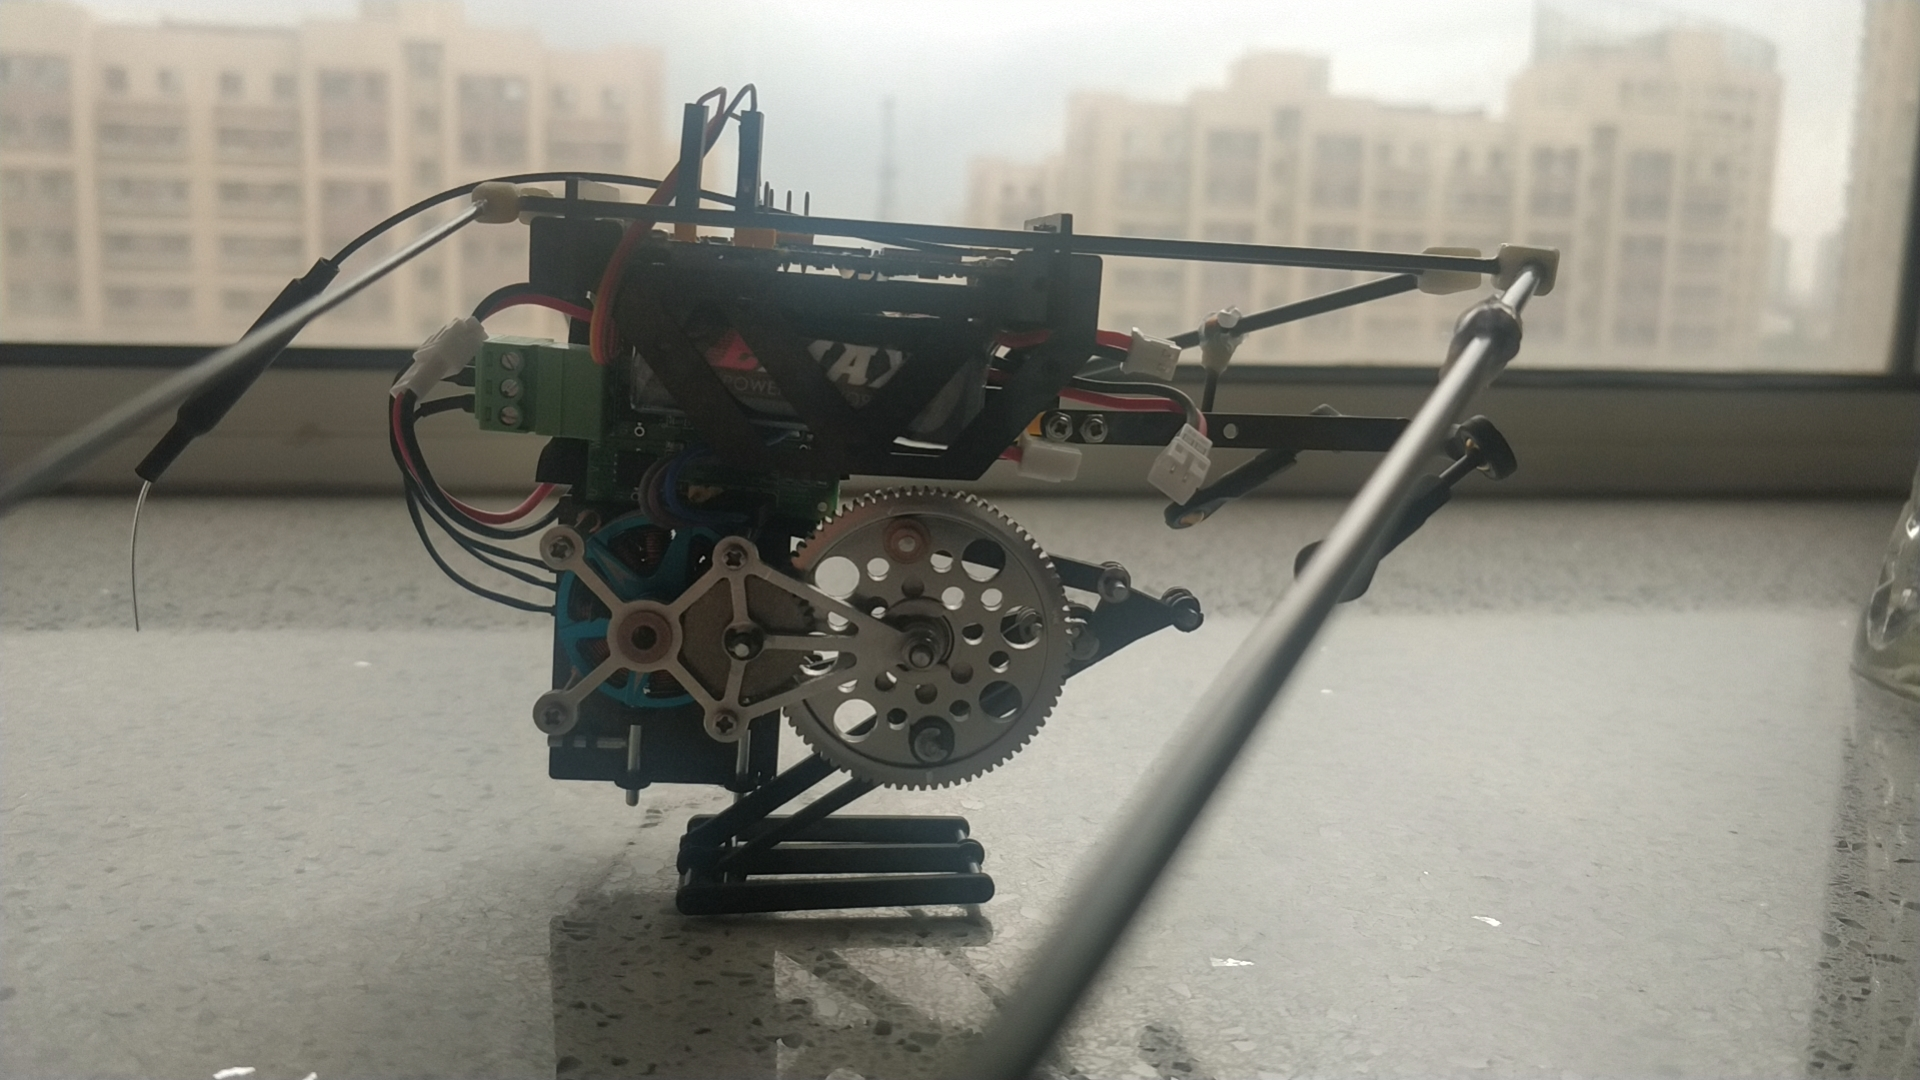
\includegraphics[height=8.5cm]{end.jpeg}
  \caption{机器人侧颜}
  \label{fig:end}
\end{figure}